\chapter{Waypoint-sampling based motion planning in wind}\label{cha:motion_planning_fw}
\section{Waypoint sampling}
The desired output of the motion planner in this thesis is a waypoint sequence $\mathcal{M}$ as defined in section \ref{sec:mission}
which takes the UAV from desired initial and final positions $\vec{p}_i$ and $\vec{p}_f$ with constraints on initial and final heading $\psi$, 
physical constraints on the UAV and wind taken into account. This formulation is well aligned with \textit{input sampling} methods such as Hybrid $A^*$ \cite{hybrid_astar}. 
In such methods, the reachability graph is created by forward simulation of the transition function $f(x, u)$ using input values $u$ sampled from a 
set $\mathcal{U}_s$. 

\subsection{State and input set definition}
Based on the kinematic model in Equation \eqref{eq:traj_model} the state vector is defined as
\begin{equation}
    x=(x_N, y_E, \psi)
\end{equation}
The input is defined as 
\begin{equation}
    u=(x_N, y_E)
\end{equation}
which is the inertial-frame coordinates of the next waypoint.
\subsection{State transition function}
Based on the definition of $u$ and the trajectory-following controller presented in Section \ref{sec:traj_controller} 
a model for the closed-loop system can be formulated. By using the closed-loop system during forward simulation, 
it is guaranteed that the controller will be able to track the resulting reference. 

The desired course for the current line-segment is
\begin{equation}
    \psi_g=\tan^{-1}(p_{E,g}/p_{N,g})
\end{equation}
By introducing a line parallel to the line-segment we can write the angle $\eta$ in Figure \ref{fig:ss_defs} as
\begin{equation}\label{eq:eta_first}
    \eta=\eta_1+\eta_2
\end{equation}
where $\eta_2$ is defined as the angle from the velocity vector $\vec{v}$ to this line. 
These angles are given by 
\begin{equation}
    \eta_2=\tan^{-1}\left(\frac{\cos\psi_g(V_a\sin\psi + W\sin\psi_w) - \sin\psi_g(V_a\cos\psi + W\cos\psi_w)}{\cos\psi_g(V_a\cos\psi + W\cos\psi_w)+\sin\psi_g(V_a\sin\psi + W\sin\psi_w)}\right)
\end{equation}
and 
\begin{equation}\label{eq:eta_last}
    \eta_1=\sin^{-1}\left(\frac{x_N\sin\psi_g-y_E\cos\psi_g}{L_1}\right)
\end{equation}
If roll dynamics are neglected, we get the resulting yaw-rate by inserting the roll command from Equation \eqref{eq:roll_cmd} into Equation \eqref{eq:traj_model}, so that 
\begin{equation}
    \dot{\psi}=\frac{a^c(x, u)}{V_a}
\end{equation}
where $a^c(x, u)$ is given by Equation \eqref{eq:lat_acc} with $\eta$ as defined in \eqref{eq:eta_first}-\eqref{eq:eta_last}.
However, in a real world case there is come maximum possible yaw-rate $\dot{\psi}_{max}$ obtainable by the system, meaning that the actual yawrate will be 
\begin{equation}\label{eq:saturation}
    \underline{\dot{\psi}}(x, u)=\begin{cases}
        a^c(x, u)/V_a & |a^c(x, u)/V_a| \leq \dot{\psi}_{max} \\
        \text{sgn}(a^c(x, u)/V_a)\dot{\psi}_{max} & \text{otherwise}
    \end{cases}
\end{equation}
Finally, the kinematic model of the closed-loop system becomes
\begin{equation}\label{eq:closed_loop}
    \dot{x}=f(x,u)=
    \begin{bmatrix}
        V_a\cos\psi + W\cos\psi_w\\
        V_a\sin\psi + W\sin\psi_w\\
        \underline{\dot{\psi}}(x, u)
    \end{bmatrix}
\end{equation}

\section{Input set generation}\label{sec:motion_prims_wind}
The concept of an input set $\mathcal{U}_s$ is closely related to the concept of motion primitives introduced in Section \ref{sec:motion_prim}. Therefore, 
the heading-change method introduced to generate motion primitives can also be applied for generating suitable inputs. The resulting set $\mathcal{U}_s$ will consist
of waypoints that result in a desired change of heading while taking UAV kinematics, wind and tracking performance of the controller into account.

The closed-loop kinematic model \eqref{eq:closed_loop} is clearly dependent on both wind speed and direction. There are several 
wind-related effects that have to be taken into account when constructing the input set.
\subsubsection{Handling different winds}
During motion planning in wind, states with any possible $\psi$ relative to the wind direction $\psi_w$ might occur. 
In practice, this means that inputs must be generated for a set of discrete wind directions $\{\psi_{w,0},\hdots,\psi_{w,n}\}$ covering 360 degrees. 
The difference between discrete directions $\psi_{w,i+1}-\psi_{w,i}$ must be small enough that the closed loop system can follow a reference trajectory in wind 
direction $\psi_w,\quad\psi_{w,i}<\psi_w<\psi_{w,i+1}$ even though $\psi_w=\psi_{w,i}$ is used in input generation.

Since the wind speed $W$ also affects the kinematic model, different input sets have to be generated for different values of $W$.
\subsubsection{Course and yaw compensation}
In the case of non-zero uniform wind, the required yaw angle $\psi$ to hold a desired 
course $\phi_d$ will be different from $\phi_d$ as shown in Section \ref{sec:straight_path_wind}. This can be compensated by 
formulating the initial and final constraints on desired course angle instead of yaw, where the course is given by 
\begin{equation}
    \psi_c(x) = \tan^{-1}\left(\frac{V_a\sin\psi + W\sin\psi_w}{V_a\cos\psi+W\cos\psi_w}\right)
\end{equation}
This also means that the initial value of $\psi$ should be set to the wind correction angle $\psi_{wca}$ as defined in Equation \eqref{eq:wca}.
\subsection{Ensuring state connectivity}
The cross-track error at the end of a line-segment can be calculated as 
\begin{equation}
    d(x_f, u) = p_{N,f}\sin\psi_g-p_{E,f}\cos\psi_g
\end{equation}
If $d(x_f, u)\neq0$ this means that $d(x_i)$ for the next line-segment will be non-zero. 
Since the closed-loop system is used when expanding the graph a small initial error can be handled.
To ensure that the value is small enough the factor $|d(x(T), u)|^2$ is added to the objective when generating inputs.
\subsection{Optimal control formulation}
Optimized inputs are defined as solutions to the optimal control problem
\begin{subequations}
    \label{eq:opt_problem_mp_uav}
    \begin{alignat}{3}
    &\min_{x(t),u,T}        &\qquad& J=|d(x(T), u)|^2 + |\psi_c(x(T))-\psi_d|^2 + \int_{0}^{T}V_a dt & \\
    &\text{subject to} & & \psi(0)=\psi_{wca} &\\
    & & & \psi_c(x(0))=0, \quad |\psi_c(x(T))-\psi_d| \leq \Delta\psi_{min} &\\
    & & & \dot{x}=f(x(t), u) &\\
    & & & x(t)\in\mathcal{X}& \\
    & & & u\in\mathcal{U} &
    \end{alignat}
\end{subequations}
for all desired values of $\psi_w$ and desired final course $\psi_d$. The final term in the objective function is equal to the distance the UAV 
travels through the air when $t\in[0, T]$. Instead of having strict equality constraints for $d(x(T), u)$ and $\psi_c(x(T))$ they 
are allowed to vary a bit from the desired values to enable some tradeoff between tracking performance, final course and distance travelled.

\subsubsection{Solving the optimal control problem}
Methods commonly used to solve optimal control problems include \textit{multiple shooting} and \textit{direct collocation} \cite{Bergman_lic}. 
However, there are some properties of \eqref{eq:opt_problem_mp_uav} which makes it hard to solve which such methods. 
One property is that the closed-loop system is highly non-linear, especially when including the saturation from Equation \eqref{eq:saturation}. 
Also, normally in optimal control problems the input $u(t)$ can be chosen freely from $\mathcal{U}$ for each time-step, while 
in this formulation the input is forced to be a constant $u(t)=u$. This means that when transformed to a Nonlinear Program using e. g. multiple shooting,
the optimization variables corresponding to $x(t)$ in each time-step all depend on the same constant $u$. 

\subsubsection{Derivative-free Optimization}
Since all other variables in Equation \eqref{eq:opt_problem_mp_uav} depend on the choice of $u$, the system can be 
simulated from the origin for different values of $u$ and the objective value $J$ calculated. Choices of $u$ which violates the constraints 
can also easily be pruned. A plot of the objective function and a simulated trajectory for the optimal $u$ is shown in Figure~\ref{fig:opt_contour}. 

\begin{figure}
    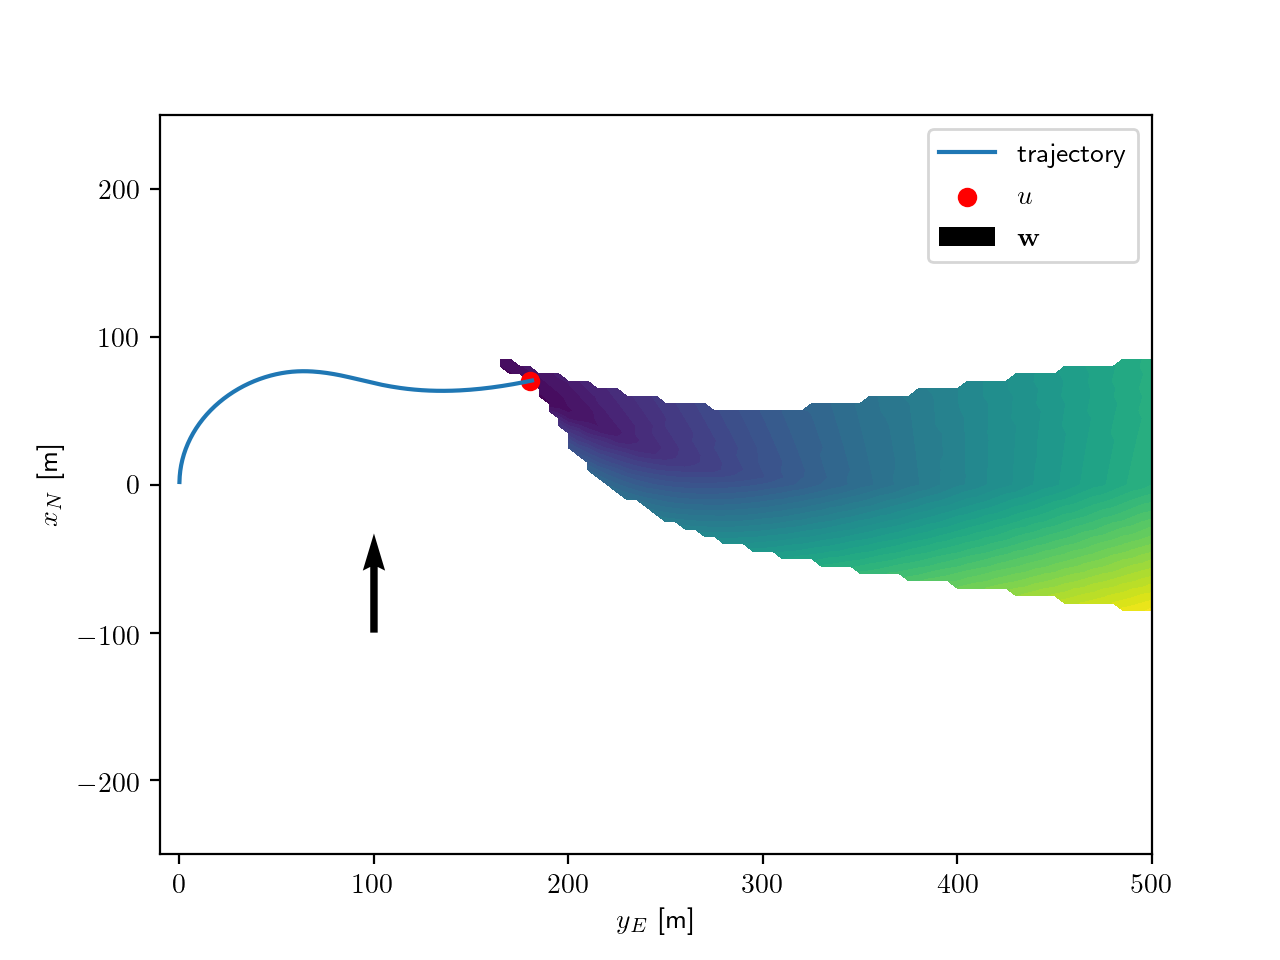
\includegraphics[width=\linewidth]{J_opt_90}
    \caption{Contour plot of optimization objective $J$ and simulated trajectory for optimal input $u$. 
    $V_a=14$ m/s, $W=5$ m/s, $\psi_w=0\degree$, $\psi_d=90\degree$, $\Delta\psi_{min}=10\degree$ and $x_i=(0, 0, 0\degree)$.}
    \label{fig:opt_contour}
\end{figure}

As can be seen there is a clear global optimum in the feasible region.  
Approximate solutions to optimization problems can be calculated by using \textit{derivative-free} optimization methods, as presented in \cite{derivative_free_opt}. 
Such methods are used to solve general optimization problems formulated as 
\begin{subequations}
    \label{eq:derivative_free_opt}
    \begin{alignat}{3}
    &\min_{x\in\reals^n}        &\qquad& f: x \rightarrow \reals & \\
    &\text{subject to} & & x\in\mathcal{X}_{feasible} &\\
    \end{alignat}
\end{subequations}
where no other information, such as the derivatives of $f$ is available.
One class of derivative-free methods, Mesh-Adaptive Direct Search (MADS) is based on creating an incrementally smaller grid around the 
currently optimal solution on which the objective function is evaluated. The quality of the solution will thus depend on having a good initial guess $x_0$ \cite{mads}.

\subsection{Guaranteeing robustness during wind variations}
In real world scenarios the wind is rarely constant. A more useful approach would thus be to generate input sets which handle wind speeds 
$W\in[W_{min},W_{max}]$. This problem can be formulated as finding an input $u$ which minimizes \eqref{eq:opt_problem_mp_uav} for both 
$W_{min}=(1-\delta_W)W$ and $W_{max}=(1+\delta_W)W$ for some $\delta_W<1$.

\subsubsection{Bi-Objective MADS}
The MADS algorithm was extended to the BiMADS algorithm in \cite{bi_mads}. This algorithm solves bi-objective optimization problems on the form 
\begin{subequations}
    \label{eq:bi_mads}
    \begin{alignat}{3}
    &\min_{x\in\reals^n}        &\qquad& F(x)=[f_1(x),f_2(x)]^T & \\
    &\text{subject to} & & x\in\mathcal{X}_{feasible} &\\
    \end{alignat}
\end{subequations}
where $f_1$ and $f_2$ are two different objectives which we wish to minimize. The solution $x^*$ of such an optimization problem 
is \textit{pareto efficient} as defined in \cite{bi_mads}, meaning that
\begin{equation}
    F(x^*+\epsilon)\succeq F(x^*)
\end{equation}
for some $\epsilon\in\reals^n$ and where $u\succeq v$ denotes that each component of $u$ is greater or equal than the corresponding component of $v$.

This formulation can be used to generate inputs by setting $f_1=J$ for $W=W_{min}$ and $f_2=J$ for $W=W_{max}$. The feasible set $\mathcal{X}_{feasible}$ is defined as 
the values of $x$ where the constraints in \eqref{eq:opt_problem_mp_uav} hold for all $W\in[W_{min},W_{max}]$.
\section{Heuristic function}
As discussed in Section \ref{sec:a-star}, the choice of heuristic function is 
crucial in achieving good performance. The goal of the heuristic function is to estimate the 
length of the shortest air-relative path from an initial state $x_i$ to a final state $x_f$.

\subsection{Cost estimation for straight line-segments}\label{sec:straight_path_heuristic}
As discussed in Section \ref{sec:straight_path_wind}, when following a straight line-segment in wind the air-relative 
distance travelled by the UAV will be different from the distance in the inertial frame. Since the yaw angle of the UAV is 
equal to $\psi_{wca}$ as defined in Equation \eqref{eq:wca}, the velocity of the UAV along the current reference line in the inertial frame is given by 
\begin{equation}
    V_{\parallel}=\cos\psi_s(V_a\cos\psi_{wca}+W\cos\psi_w) + \sin\psi_s(V_a\sin\psi_{wca}+W\sin\psi_w)
\end{equation}
This means that the time travelled by the UAV is equal to 
\begin{equation}
    t=\frac{\|\vec{p}_{i+1}-\vec{p}_i\|}{V_\parallel}
\end{equation}
where $\vec{p}_{i}$ and $\vec{p}_{i+1}$ are the start and end points of the line in inertial coordinates. Thus, the distance 
travelled in the air-relative frame is equal to 
\begin{equation}
    s_A=V_at=\frac{V_a}{V_\parallel}\|\vec{p}_{i+1}-\vec{p}_{i}\|
\end{equation}
and $s_A$ provides a good heuristic estimate for traveling along a straight path segment assuming that $\psi(x_i)=\psi(x_f)=\psi_{wca}$.
This also means that the euclidean distance $\|\vec{p}_{i+1}-\vec{p}_{i}\|$ is a non-admissible heuristic if 
$V_a/V_\parallel<1$.

\subsection{Cost estimation for arbitrary initial and final heading}
\todo[inline]{Förbättra projektionsmetoden (garantera admissible?)}
Estimating the cost for traveling between states with arbitrary $\psi_i$ and $\psi_f$ is a more challenging problem than straight line-segments.
Methods to calculate time-optimal such paths in the presence of wind are given in both \cite{optimal_path_target} and \cite{optimal_path_trochoidal}, 
but since there is no analytical solution in all cases these methods rely on numerical root-finding techniques.
Computing these values every time an heuristic estimate is needed was assumed too computationally expensive.

When the heuristic cannot be calculated in real-time, another option is to use a HLUT as discussed in Section \ref{sec:hlut}. By using the generated 
inputs $\mathcal{U}_s$ when calculating costs stored in the HLUT these will be perfect estimations of the heuristic value. However, a drawback of 
using a HLUT is that the wind speed $W$ affects cost, and thus different $W$ require different HLUTs. 

To estimate the cost of queries not stored in the HLUT, these queries can be projected as shown in Figure \ref{fig:hlut_proj}. The total heuristic value can then be estimated as 
\begin{equation}
    h'(x, x_f) = h_{HLUT}(x, x_p) + h_s(x_p, x_f)
\end{equation}
where $h_s(x, x')$ is the estimated cost for a straight line-segment.
\begin{figure}
    \begin{center}
        \begin{tikzpicture}
            \draw (-2, -2) rectangle (2, 2);

            \draw[my_v] (0,0) -- node[at end, below]{$y_E$} (1,0);
            \draw[my_v] (0,0) -- node[at end, left]{$x_N$} (0,1);

            \node[point] at (0,0){};
            \node[below] at (0,0){$x$};

            \node[point] at (2,1){};
            \node[above] at (2,1){$x_p$};
            \draw (0,0) -- node[midway, below, anchor=north west]{$h_{HLUT}(x, x_p)$} (2,1);

            \node[point] at (4,2){};
            \node[above] at (4,2){$x_f$};
            \draw[dashed] (2,1) -- node[midway,below, anchor=north west]{$h_s(x_p,x_f)$} (4,2);

            \node[anchor=west] at (-1.8,-1.75){HLUT available};
        \end{tikzpicture}
    \end{center}
    \caption{Projection of queries on HLUT}
    \label{fig:hlut_proj}
\end{figure}

\subsubsection{Effects of wind variations on heuristic}
If the actual wind speed $W'$ is different from the wind speed $W$ used during planning this 
might affect the admissibility of the heuristic and in turn the optimality guarantees of the planner. 
Consider traveling along a straight path segment of length $\Delta s=\|x-x'\|$ under the assumptions in Section \ref{sec:straight_path_wind}. 
An admissible heuristic is then 
\begin{equation}
    h'(x, x')=\frac{V_a}{V}\Delta s
\end{equation}
where $V$ is the velocity in the inertial frame. Wind has the largest effect on $V$ if the path is in downwind or upwind, and in those cases $V=V_a\pm W'$. The 
heuristic function $h(x, x')$ used during planning is the same but with $V=V_a\pm W$. The ratio between the admissible and actual heuristics become 
\begin{equation}\label{eq:wind_heuristic_eps}
    \epsilon = \frac{h}{h'} = \frac{V_a \pm W'}{V_a \pm W}
\end{equation}
where the signs in the numerator and denominator must be equal. From Section \ref{sec:sub_optimal} we know that optimality guarantees are lost if 
$\epsilon>1$ which is the case if $W'>W$ when traveling downwind, or $W'<W$ when traveling upwind. However, the length of the resulting path is 
guaranteed to be within a factor $\epsilon$ of the optimal length. Moreover, the effects of using an incorrect wind estimate will be more significant if the 
magnitude of $W'$ is close to that of $V_a$.